\documentclass{standalone}
\usepackage{tikz}
\usepackage{fontenc}
\usetikzlibrary{arrows, shapes.multipart, positioning,automata}


\begin{document}
	
	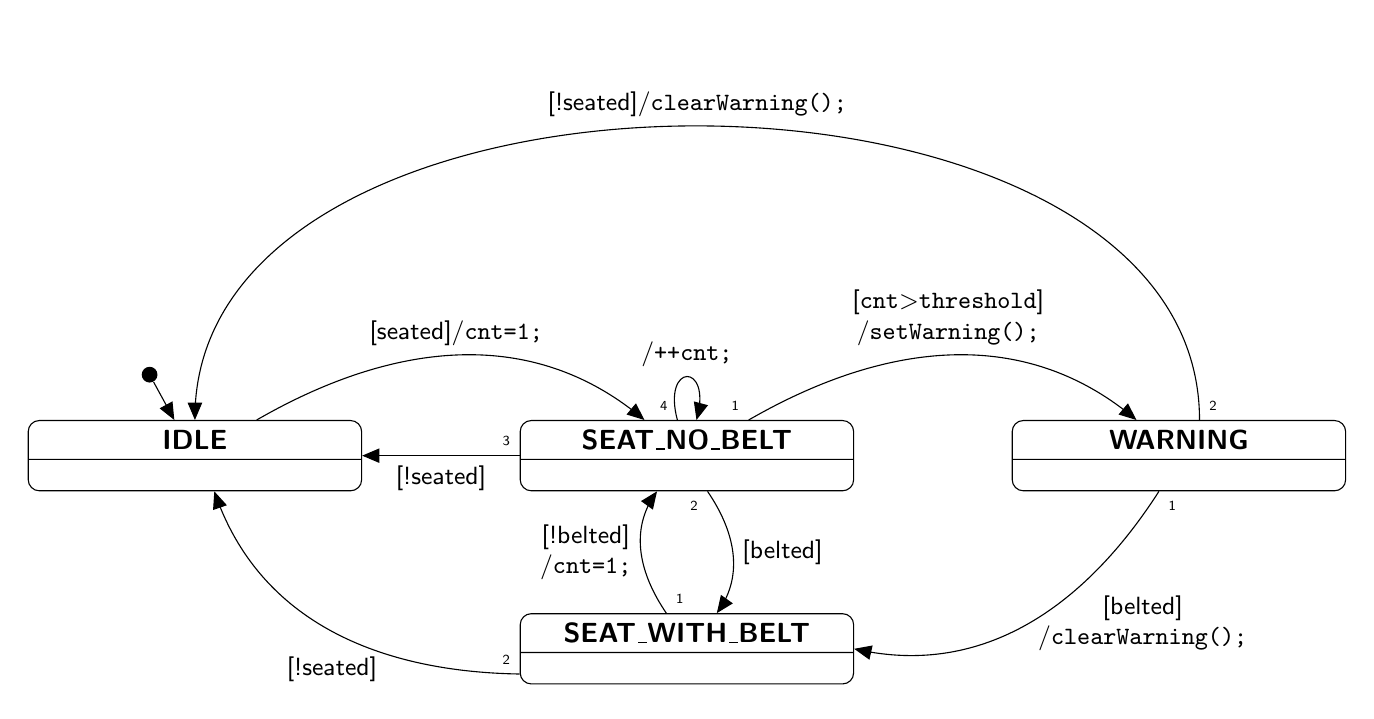
\begin{tikzpicture} %
		[
			font={\sffamily},
			every text node part/.style={align=center}, % sleeky thing behind nodeparts...
			state/.style={
				anchor=center,
				draw,
				rectangle split,
				rectangle split parts=2, 
				rectangle split part align={center, flushed left},
				rounded corners=4,
				minimum width=4.2 cm,%text centered,
				text width= 4 cm,
				node distance= 2 cm,
			},
			arch/.style={-triangle 45},
			transit/.style={font={\small \sffamily},midway},
			active/.style={red},
			stdBend/.style={bend left, in =140},
			priority/.style={font={\tiny \sffamily}},
		]
		\node[state] (s0) {\textbf{IDLE}};
		\node[state, right =of s0] (s1) {\textbf{SEAT\textunderscore NO\textunderscore BELT}};
		\node[state, below =of s1.center] (s2) {\textbf{SEAT\textunderscore WITH\textunderscore BELT}};
		\node[state, right =of s1] (s3)
		{\textbf{WARNING}};
		\node[circle,inner sep=0, minimum size=2mm, fill=black](init)[above left =5mm and 5mm of s0.north]{};
		
		\draw[arch] (init) -- (s0.120);
		
		\draw[arch] (s0) 
			to [stdBend] node[transit,above]{[seated]/\texttt{cnt=1;}} 
			(s1);
		\draw[arch] 
			(s1) 
			to [stdBend] node[transit,above]{[\texttt{cnt\textgreater threshold}]\\/\texttt{setWarning();}}  node [pos=0,above left,priority]{1}
			(s3);
		\draw[arch] 
			(s1) 
			to [loop above] node[transit,above]{/\texttt{++cnt;}}  
			node [pos=0,above left,priority]{4}
			(s1);
		\draw[arch] 
		(s1) 
		to [stdBend] node[transit,right]{[belted]} node [pos=0,below left,priority]{2}
		(s2);
		\draw[arch] 
		(s2) 
		to [stdBend] node[transit,left]{[!belted]\\/\texttt{cnt=1;}} node [pos=0,above right,priority]{1}
		(s1);
		\draw[arch] 
		(s1.west) 
		-- node[transit,below]{[!seated]} node [pos=0,above left,priority]{3}
		(s0.east);
		\draw[arch] 
		(s2) 
		to [stdBend] node[transit,below = 2mm]{[!seated]} node [pos=0,above left,priority]{2}
		(s0);
		% would this happen?...
		\draw[arch]
		(s3)
		to [stdBend] node[transit,right]{[belted]\\/\texttt{clearWarning();}} 
		node [pos=0,below right,priority]{1}
		(s2.east);
		\draw[arch]
		(s3.60)
		to [out = 90, in = 90] node[transit,above]{[!seated]/\texttt{clearWarning();}} 
		node [pos=0,above right,priority]{2}
		(s0);
	\end{tikzpicture}	
\end{document}